% !TEX root = ../main.tex

% Local Variables:
% TeX-master: "../main"
% End:
% chktex-file 26

%%%%%%%%%%%%%%%%%%%%%%%%%%%%%%% Header %%%%%%%%%%%%%%%%%%%%%%%%%%%%%%%%%%%%%%%%%%%%
\begin{minipage}[l]{0.42\textwidth}
    
\includegraphics[width=1\textwidth]{img/logo-UNAMBA.png}
\end{minipage}
\hfill
\begin{minipage}[c]{0.5\textwidth}
    \begin{flushright}
	\large{\textbf{Unidad \#2}}\\
	\large{Lectures on Física I}\\
	\large{24 de Julio del 2025. Haquira, Apurimac}\\
        % \large{\textbf{Student:} Huallpa Aimituma Josué David}
    \end{flushright}
\end{minipage}
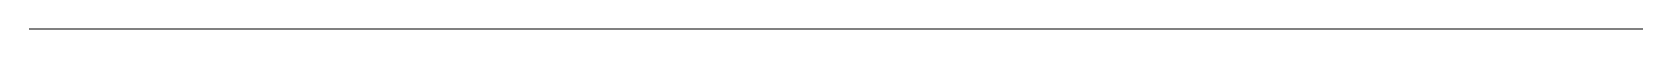
\begin{tikzpicture}
    \draw[gray,thick] (-6.5,0)--(14,0);
\end{tikzpicture}


 %%%%%%%%%%%%%%%%%%%%%%%% INICIO DEL CONTENIDO EN DOS COLUMNAS %%%%%%%%%%%%%%%%%%%%%

 \begin{multicols}{2}
     \begin{center}
         \LARGE{\textbf{Capítulo IV: Cinemática del punto}}\\	
         \vspace{0.2cm}
         % \Large {Lecturers Esteban Chalbaud \& Daniel Galviz} \\
         % \large{Teaching Assistant: Mauricio Gamonal \& Irvin Martínez}\\
         % \large{PhysicsLatam.com}\\
         % \vspace{0.2cm}
         \large{Fecha de entrega: 07 Agosto 2025, 5:59 pm (GMT-4)}\\
         % \vspace{0.2cm}
         \large{— Evaluación Parcial 2 —}
     \end{center}
          %%%%%%%%%%%%%%%%%%%%%%%%%%%%excercise%%%%%%%%%%%%%%%%%%%%%%%%%%%%%%%%%%%%%%%%
     \begin{excercise}[][][a) $t_1=2 \ \mathrm{s}$, $t_2=3\ \mathrm{s}$, $x(t=2)=-23 \ \mathrm{m}$, $x(t=3)=0 \ \mathrm{m}$, $a(t=2)=-6 \ \mathrm{ms^{-2}}$, $a(t=3)=6 \ \mathrm{ms^{-2}}$ , b) $v(t=3)=18 \ \mathrm {ms^{-1}}$, c) $a=-6 \ \mathrm{ms^{-2}}$]{ex:k0}{
        \textbf{(Mov. Rectilineo no Uniforme)}\\
        El movimiemto de una partícula esta definida por:
        \begin{equation*}
            x(t)=2t^3-15t^2+36t-27
        \end{equation*}
        \begin{itemize}
            \item[a)] Calcular el tiempo, posición y aceleración cuando la velocidad vale cero.
            \item[b)] Hallar la velocidad instantanea para $t=3$
            \item[c)] Hallar la aceleración ,edoa entre $x(t=1)$ y $x(t=3)$
        \end{itemize}
         }
     \end{excercise} 
     %%%%%%%%%%%%%%%%%%%%%%%%%%%%excercise%%%%%%%%%%%%%%%%%%%%%%%%%%%%%%%%%%%%%%%%
     \begin{excercise}[][][$v(t) = \displaystyle{4t-\frac{t^3}{3}-1}\ (\mathrm{ms^{-1}})$, $x(t)=\displaystyle{2t^4-\frac{t^4}{12}-t-\frac{3}{4}} \ (\mathrm{m})$]{ex:k1}{
         La aceleración de un cuerpo que se mueve a lo largo de una linea recta está dado por
         \begin{equation*}
             a(t)=4-t^2 
         \end{equation*}
         Encontrar las expresiones para la velocidad y el desplazamiento como funciones del tiempo si cuando $t=3 \ \mathrm{s}$, $v(t)=2 \ \mathrm{ms^{-1}}$, $x(t)=9 \ \mathrm{m}$
         }
     \end{excercise}   
     %%%%%%%%%%%%%%%%%%%%%%%%%%%%excercise%%%%%%%%%%%%%%%%%%%%%%%%%%%%%%%%%%%%%%%%
    \begin{excercise}[][][a) $x = 47.58 \mathrm{m}$; b) $a=51 \ (\mathrm{ms^{-2}})$]{ex:k2}{
         Un cuerpo se mueve a lo largo de una linea recta de acuerdo a la ley 
         \begin{equation*}
             v(t)=t^3+4t^2+2
         \end{equation*}
         Si x=4 m cuando $t=2\ \mathrm{s}$,
            \begin{itemize}
                \item[a)] Encontrar el valor de x cuando  $t=3 \ \mathrm{s}$,
                \item[b)] Encontrar  su aceleracion
            \end{itemize}
        }
    \end{excercise}      
    %%%%%%%%%%%%%%%%%%%%%%%%%%%%excercise%%%%%%%%%%%%%%%%%%%%%%%%%%%%%%%%%%%%%%%%
    \begin{excercise}[][][$v(x) = \sqrt{16-2x^2}$]{ex:k3}{
         Un cuerpo se mueve a lo largo de una linea recta, su aceleración esta dada por 
         \begin{equation*}
             a(x)=-2x 
         \end{equation*}
         donde $x$ esta en metros y $a$ en $\mathrm{ms^{-2}}$ Encontrar la relación entre la velocidad y la distancia, suponiendo que cuando $x=0$,  $v=4 \ \mathrm{ms^{-1}}$.
         }
    \end{excercise}
    %%%%%%%%%%%%%%%%%%%%%%%%%%%%excercise%%%%%%%%%%%%%%%%%%%%%%%%%%%%%%%%%%%%%%%%
    \begin{excercise}[][][a) $v(t) = \displaystyle{\frac{v_0}{1+kv_0t}}$, $x(t)=x_0+\displaystyle{\frac{1}{k}}\ln(1+kv_0t)$; b) $v(x)=\displaystyle{v_0e^{-k(x-x_0)}}$]{ex:k4}{
         La aceleración de un cuerpo que se mueve a lo largo de una línea recta está dada por
         \begin{equation*}
             a(x)=-kv^2 
         \end{equation*}
         donde $k$ es una constante, suponiendo que cuando $t=0$,  $v=v_0$.
         \begin{itemize}
             \item[a)] Encontrar la velocidad y el desplazamiento en función del tiempo.
             \item[b)] Encontrar también x en función de t y  v en función de x.
         \end{itemize}
        }
    \end{excercise}
    %%%%%%%%%%%%%%%%%%%%%%%%%%%%excercise%%%%%%%%%%%%%%%%%%%%%%%%%%%%%%%%%%%%%%%%
\begin{excercise}[][][a) $v(t) = \displaystyle{8-4e^{4-t}}$, $x(t)=\diplaystyle{8t+e^{-4t}}-1$; b) $x(v)=\displaystyle{-2\ln{(8-v)}-\frac{v}{4}+4\ln 2+1}$]{ex:k5}{
         Para un cuerpo en movimiemto rectilineo cuya aceleración esta dada por 
         \begin{equation*}
             a(x)=32-4v
         \end{equation*}
         las condiciones iniciales son $x=0$,  $v=4$ para $t=0$.
         \begin{itemize}
             \item[a)] Encontrar la velocidad y el desplazamiento en función del tiempo.
             \item[b)] Encontrar también x en función de t y  v en función de x.
         \end{itemize}
        }
    \end{excercise}
     %%%%%%%%%%%%%%%%%%%%%%%%%%%%excercise%%%%%%%%%%%%%%%%%%%%%%%%%%%%%%%%%%%%%%%%
     \begin{excercise}[][][a) $v = 25\ (\mathrm{ms^{-1}})$, b) $v = 20.5\ (\mathrm{ms^{-1}})$, c) $v = 20.005\ (\mathrm{ms^{-1}})$, d) $v = 20.00005\ (\mathrm{ms^{-1}})$, e) $v = 20\ (\mathrm{ms^{-1}})$,]{ex:k6}{
        \textbf{(MRU - MRUV)}\\
        Una partícula se mueve a lo largo del eje x de manera que su posición en cualquier instante t está dado por 
        \begin{equation*}
            x(t)=5t^2+1 
        \end{equation*}
        donde x se expresa en metros y t segundos. Calcular su velocidad media en el intervalo de tiempo entre (a) 2 s y 3 s, (b) 2 s y 2,1 s, (c) 2 s y 2,001 s, (d) 2 s y 2,00001 s. Calcular también (e) la velocidad instantánea a los 2 s.
         }
     \end{excercise} 


      %%%%%%%%%%%%%%%%%%%%%%%%%%%%excercise%%%%%%%%%%%%%%%%%%%%%%%%%%%%%%%%%%%%%%%%
    \begin{excercise}[][][a) $v=31\ \mathrm{ms^{-1}}$,  $x=19\ \mathrm{m}$; b)  $v=-255\ \mathrm{ms^{-1}}$,  $x=77\ \mathrm{m}$;]{ex:k8}{
            Un cuerpo se mueve con una velocidad inicial de $3\  \mathrm{m s^-1}$, y una aceleración constante de $4 \ \mathrm{ m s^{-2}}$ en la misma dirección que la de la velocidad. 
            \begin{itemize}
                \item[a)]  ¿Cuál es la velocidad del cuerpo y la distancia recorrida al final de 7 s?                 
                \item[b)] Resolver el mismo problema para un cuerpo cuya aceleración tiene dirección opuesta de la velocidad.                
                \item[c)]  Escribir la expresión del desplazamiento en función del tiempo.
            \end{itemize}           
         }
    \end{excercise}
    
    %%%%%%%%%%%%%%%%%%%%%%%%%%%%excercise%%%%%%%%%%%%%%%%%%%%%%%%%%%%%%%%%%%%%%%%
     \begin{excercise}[][][$2.25\times 10^{14}\ \mathrm{ms^{-2}}$]{ex:k7}{
            Un electrón incide sobre una pantalla de televisión con una velocidad de $3 \times 10^{6}\ \mathrm{ m s^-1}$. Suponiendo que ha sido acelerado desde el reposo a través de una distancia de 0.04 m, encontrar su aceleración promedio. 
         }
    \end{excercise}
    %%%%%%%%%%%%%%%%%%%%%%%%%%%%excercise%%%%%%%%%%%%%%%%%%%%%%%%%%%%%%%%%%%%%%%%
    \begin{excercise}[][][a) $v_0=80\ \mathrm{ms^{-1}}$ b)  $a=5.33\ \mathrm{ms^{-2}}$,  $x=77\ \mathrm{m}$;]{ex:k9}{
            Un aeoroplano, al partir, recorre 600 m, en 15 s. Suponiendo una aceleración constante              
            \begin{itemize}
                \item[a)] Calcular la velocidad de partida.               
                \item[b)] Calcular también la aceleración en  $\mathrm{ m s^{-2}}$.
            \end{itemize}
         }
    \end{excercise}
    %%%%%%%%%%%%%%%%%%%%%%%%%%%%excercise%%%%%%%%%%%%%%%%%%%%%%%%%%%%%%%%%%%%%%%%
    \begin{excercise}[][][a) $a=4000\ \mathrm{m min^{-2}}$,  $x=125\ \mathrm{m}$; b)  $t=5\ \mathrm{s}$,  $x=223\ \mathrm{m}$;]{ex:k10}{
            Un automóvil, que parte del reposo, alcanza una velocidad de $60  \ \mathrm{ km h^{-1}}$ en 15 s. 
            \begin{itemize}
                \item[a)] Calcular la aceleración promedio en $\ \mathrm{ m min^{-2}}$ y la distancia recorrida.               
                \item[b)] Suponiendo que la aceleración es constante, ¿cuántos segundos más le tomará al auto para alcanzar los $80  \ \mathrm{ km h^{-1}}$? ¿Cuál ha sido la distancia total recorrida?             
            \end{itemize} 
         }
    \end{excercise}
    %%%%%%%%%%%%%%%%%%%%%%%%%%%%excercise%%%%%%%%%%%%%%%%%%%%%%%%%%%%%%%%%%%%%%%%
    \begin{excercise}[][][a) $x=9.25\ \mathrm{m}$]{ex:k11}{
            Un auto parte del reposo y se desplaza con una aceleración de $1\  \mathrm{ms^{-2}}$ durante 1 s. Luego se apaga el motor y el auto desacelera debido a la fricción, durante 10 s a un promedio de $5 \mathrm{cms^{-2}}$. Entonces se aplican los frenos y el auto se detiene en 5 segundos más.             \begin{itemize}
                \item[a)] Calcular la distancia total recorrida por el auto.              
                \item[b)] Hacer un gráfico de x, v y a contra t.
            \end{itemize}
         }
    \end{excercise}
    %%%%%%%%%%%%%%%%%%%%%%%%%%%%excercise%%%%%%%%%%%%%%%%%%%%%%%%%%%%%%%%%%%%%%%%
    \begin{excercise}[][][ $x=209\ \mathrm{m}$]{ex:k12}{
            Un auto parte del reposo y se mueve con una aceleración de $4\ \mathrm{ms^{-2}}$ y viaja durante 4 s. Durante los próximos 10 s se mueve con movimiento uniforme. Se aplican luego los frenos y el auto desacelera a razón de $8\ \mathrm{ms^{-2}}$ hasta que se detiene. Hacer un gráfico de la velocidad contra el tiempo y demostrar que el área comprendida entre la curva y el eje del tiempo mide la distancia total recorrida. 
         }
    \end{excercise}
    %%%%%%%%%%%%%%%%%%%%%%%%%%%%excercise%%%%%%%%%%%%%%%%%%%%%%%%%%%%%%%%%%%%%%%%
    \begin{excercise}[][][$d=180\ \mathrm{m}$,  $t=18\ \mathrm{s}$]{ex:k13}{
         Un auto está esperando que cambie la luz roja. Cuando la luz cambia a verde, el auto acelera uniformemente durante 6s a razón de $2 \ \mathrm{ms^{-2}}$, después de lo cual se mueve con velocidad constante. En el instante que el auto comienza a moverse, un camión que se mueve en la misma dirección con movimiento uniforme de $10 \ \mathrm{ms^{-1}}$, lo pasa. ¿En qué tiempo, y a qué distancia se encontrarán nuevamente el auto y el camión? 
         }
    \end{excercise}
    %%%%%%%%%%%%%%%%%%%%%%%%%%%%excercise%%%%%%%%%%%%%%%%%%%%%%%%%%%%%%%%%%%%%%%%
    \begin{excercise}[][][a) $t=103\ \mathrm{s}$]{ex:k14}{
         Dos autos, A y B, se mueven en la misma dirección. Cuando t = 0, sus velocidades respectivas son  $1 \ \mathrm{fts^{-1}}$ y  $3 \ \mathrm{fts^{-1}}$, y sus respectivas aceleraciones son  $2 \ \mathrm{fts^{-2}}$ y  $1 \ \mathrm{fts^{-2}}$. Si el auto A se encuentra 1,5 ft delante del auto B cuando t = 0, calcular cuándo se encontrarán lado a lado. 
         }
    \end{excercise}
    %%%%%%%%%%%%%%%%%%%%%%%%%%%%excercise%%%%%%%%%%%%%%%%%%%%%%%%%%%%%%%%%%%%%%%%
    \begin{excercise}[][][a) $x=10\ \mathrm{m}$; b) $t=8/3\ \mathrm{s}$; c)  $v=4\ \mathrm{ms^{-1}}$; d)  $v=16-12t_0-6\Delta t$; e) $v(t)16-12t$; f)  $v=16\ \mathrm{ms^{-1}}$; g)  $t=41.33\ \mathrm{s}$,  $x=10.7\ \mathrm{m}$; h)  $a=-12\ \mathrm{ms^{-2}}$;  i)  $a(t)=-12\ \mathrm{ms^{-2}}$]{ex:k15}{
         Un cuerpo se está moviendo a lo largo de una recta de acuerdo a la ley
            \begin{equation*}
              x(t)=16t-6t^2  
            \end{equation*}
         donde x se mide en metros y t en segundos. 
        \begin{itemize}
            \item[a)] Encontrar la posición del cuerpo cuando $t = 1$ s.  
            \item[b)] ¿Para qué tiempos el cuerpo pasa por el origen?
            \item[c)] Calcular la velocidad promedio para el intervalo de tiempo $0 <t<2$ s.    
            \item[d)] Encontrar la expresión general de la velocidad promedio en el intervalo $t_0 < t < (t_0 + \Delta t)$. 
            \item[e)] Calcular la velocidad en cualquier instante.
            \item[f)] Calcular la velocidad instantánea para $t=0$.
            \item[g)] ¿Para qué tiempos y posiciones estará el cuerpo estacionario? 
            \item[h)] Encontrar la expresión general de la aceleración promedio para el intervalo de tiempo $t_0 <t < (t_0 + \Delta t)$.
            \item[i)] Encontrar la expresión general de la aceleración instantánea en cualquier instante. 
            \item[j)] ¿Para qué tiempos es la aceleración instantánea cero? 
            \item[k)] Representar en un conjunto simple de ejes x contra t, v contra t, y a contra t. 
            \item[l)]  ¿Para qué tiempo(s) el movimiento es acelerado y para qué tiempo(s) es retardado? 
        \end{itemize}
        }
    \end{excercise}
    %%%%%%%%%%%%%%%%%%%%%%%%%%%%excercise%%%%%%%%%%%%%%%%%%%%%%%%%%%%%%%%%%%%%%%%
    \begin{excercise}[][][a) $v=-110\ \mathrm{ms^{-1}}$,  $x=610\ \mathrm{m}$; b)  $v=-86\ \mathrm{ms^{-1}}$,  $x=-370\ \mathrm{m}$;]{ex:k16}{
         \textbf{(Caida Libre)}\\ 
         Una piedra cae desde un globo que desciende a una velocidad uniforme de $12\  \mathrm{ms^{-1}}$. 
            \begin{itemize}
                \item[a)] Calcular la velocidad y la distancia recorrida por la piedra después de 10 s. 
                \item[b)] Resolver el mismo problema para el caso cuando el globo se eleva a la misma velocidad.
            \end{itemize}
        }
    \end{excercise}
    %%%%%%%%%%%%%%%%%%%%%%%%%%%%excercise%%%%%%%%%%%%%%%%%%%%%%%%%%%%%%%%%%%%%%%%
    \begin{excercise}[][][$t=1.43\ \mathrm{s}$; $x=18.6\ \mathrm{m}$]{ex:k17}{
         Una piedra se lanza verticalmente hacia arriba con una velocidad de  $20\  \mathrm{ms^{-1}}$. ¿Cuándo tendrá una velocidad de  $6\  \mathrm{ms^{-1}}$. y a qué altura se encontrará?  
         }
    \end{excercise}
    %%%%%%%%%%%%%%%%%%%%%%%%%%%%excercise%%%%%%%%%%%%%%%%%%%%%%%%%%%%%%%%%%%%%%%%
    \begin{excercise}[][][a) $v=227.2\ \mathrm{fts^{-1}}$,  $t_1=14.6\ \mathrm{s}$,  $t_2=0.4\ \mathrm{s}$;]{ex:k18}{
         Se tira una piedra hacia arriba desde el fondo de un pozo de 88 ft de profundidad con una velocidad inicial de $240 \ \mathrm{fts^{-1}}$. Calcular el tiempo que demorará la piedra en alcanzar el borde del pozo, y su velocidad. Discutir las respuestas posibles. 
         }
    \end{excercise}
    %%%%%%%%%%%%%%%%%%%%%%%%%%%%excercise%%%%%%%%%%%%%%%%%%%%%%%%%%%%%%%%%%%%%%%%
    \begin{excercise}[][][a) $h_{\mathrm{max}}=25\ \mathrm{ft}$, b) $h=119\ \mathrm{ft}$; c)  $v=99\ \mathrm{fts^{-1}}$]{ex:k19}{
         Un hombre parado en el techo de un edificio tira una bola verticalmente hacia arriba con una velocidad de  $40 \ \mathrm{fts^{-1}}$. La bola llega al suelo 4,25 s más tarde. 
            \begin{itemize}
                \item[a)] ¿Cuál es la máxima altura alcanzada por la bola? 
                \item[b)] ¿Qué altura tiene el edificio? 
                \item[c)] ¿Con qué velocidad llegará la bola al suelo ?
            \end{itemize}
         }
    \end{excercise}
    %%%%%%%%%%%%%%%%%%%%%%%%%%%%excercise%%%%%%%%%%%%%%%%%%%%%%%%%%%%%%%%%%%%%%%%
    \begin{excercise}[][][$h=900\ \mathrm{ft}$,  $t=7.5\ \mathrm{s}$]{ex:k20}{
         Un cuerpo que cae recorre 224 ft en el último segundo de su movimiento. Suponiendo que el cuerpo partió del reposo, determinar la altura desde la cual cayó el cuerpo y qué tiempo le tomó llegar al suelo. 
         }
    \end{excercise}
    %%%%%%%%%%%%%%%%%%%%%%%%%%%%excercise%%%%%%%%%%%%%%%%%%%%%%%%%%%%%%%%%%%%%%%%
    \begin{excercise}[][][]{ex:k21}{
         Una piedra es lanzada verticalmente hacia arriba desde el techo de un edificio con una velocidad de $29.4 \ \mathrm{ms^{-1}}$. Otra piedra se deja caer 4 s después que se lanza la primera. Demostrar que la primera piedra pasará a la segunda exactamente 4 s después que se soltó la segunda. 
         }
    \end{excercise}
      %%%%%%%%%%%%%%%%%%%%%%%%%%%%excercise%%%%%%%%%%%%%%%%%%%%%%%%%%%%%%%%%%%%%%%%
    \begin{excercise}[][][$t=18\ \mathrm{s}$;]{ex:k22}{
         Un cuerpo se deja caer y simultáneamente un segundo cuerpo, se tira hacia abajo con una velocidad inicial de $100 \ \mathrm{cms^{-1}}$. ¿Cuándo será la distancia entre ellos de 18 m?
         }
    \end{excercise}
    %%%%%%%%%%%%%%%%%%%%%%%%%%%%excercise%%%%%%%%%%%%%%%%%%%%%%%%%%%%%%%%%%%%%%%%
    \begin{excercise}[][][a) $v=31\ \mathrm{ms^{-1}}$,  $x=19\ \mathrm{m}$; b)  $v=-255\ \mathrm{ms^{-1}}$,  $x=77\ \mathrm{m}$;]{ex:k23}{
        \textbf{(Mov. Curvilineo)}\\ 
        1
        }
    \end{excercise}
    %%%%%%%%%%%%%%%%%%%%%%%%%%%%excercise%%%%%%%%%%%%%%%%%%%%%%%%%%%%%%%%%%%%%%%%
    \begin{excercise}[][][a) $\vec{r}=(t^4+2t^2+1)\vec{\imath}+(2t+2)\vec{\jmath}\ \mathrm{m}$, b)  $y^2=4x$;]{ex:k24}{
         Un punto se mueve en el plano XY de tal manera que:
            \begin{equation*}
                \vec{v}=(4t^3+4t)\vec{\imath}+4t\vec{\jmath}
            \end{equation*}
         Si el vector posición del punto es:
            \begin{equation*}
                \vec{r}=\vec{\imath}+2\vec{\jmath}
            \end{equation*}
        cuando t=0, encontrar:
        \begin{itemize}
            \item[a)] El vector posición para cualquier t.
            \item[b)] La ecuación de la trayectoria.
        \end{itemize}
         }
    \end{excercise}
    %%%%%%%%%%%%%%%%%%%%%%%%%%%%excercise%%%%%%%%%%%%%%%%%%%%%%%%%%%%%%%%%%%%%%%%
\begin{excercise}[][][a) $\vec{r}=(4\sin t +4t)\vec{\imath}-(3\cos t+3)\vec{\jmath}\ \mathrm{m}$, b)  $x=(4\sin t +4t$, $y=-(3\cos t+3)$; c) $\vec{v}=6.84\vec{\imath}+2.12\vec{\jmath}$]{ex:k25}{
         Una particula se mueve en el plano XY de acuerdo a 
        \begin{equation*}
                \vec{a}=-4\sin t\vec{\imath}+4\cos t\vec{\jmath}
            \end{equation*}
            Si cuando t=0, $\vec{r}=3\vec{\jmath}$ y $\vec{v}=4\vec{\imath}$, encontrar:
        \begin{itemize}
            \item[a)] El vector posición para cualquier t.
            \item[b)] La ecuación de la trayectoria.
            \item[c)] El valor de la velocidad cuando $t=\pi/4$ s.
        \end{itemize}
         }
    \end{excercise}
    %%%%%%%%%%%%%%%%%%%%%%%%%%%%excercise%%%%%%%%%%%%%%%%%%%%%%%%%%%%%%%%%%%%%%%%
    \begin{excercise}[][][a) $\vec{r}=(3t^2-t +1)\vec{\imath}-2 e^{-3t}\vec{\jmath} + 2\cos (4t)\vec{k}$]{ex:k26}{
         Una particula se mueve con una aceleración:
        \begin{equation*}
            \vec{a}=6\vec{\imath}-18 e^{3t}\vec{\jmath}-32\cos{(4t)}\vec{k}
            \end{equation*}
            Si cuando t=0, $\vec{r}=3\vec{\jmath}$ y $\vec{v}=4\vec{\imath}$, encontrar:
        \begin{equation*}
            \vec{v}(0)=-\vec{\imath}+6\vec{\jmath}
        \end{equation*}
        \begin{equation*}
            \vec{r}(0)=\vec{\imath}-2\vec{\jmath}+ 2\vec{k}
        \end{equation*}
        Calcular
        \begin{itemize}
            \item[a)] El vector posición para cualquier t.
            \item[b)] La ecuación de la trayectoria.
        \end{itemize}
         }
    \end{excercise}
    %%%%%%%%%%%%%%%%%%%%%%%%%%%%excercise%%%%%%%%%%%%%%%%%%%%%%%%%%%%%%%%%%%%%%%%
    \begin{excercise}[][][a) $\vec{e}_t=\frac{1}{\sqrt{t^2+8}}(t\vec{\imath}+2\vec{\jmath}-2\vec{k})$, b) $\rho=\sqrt{\frac{(t^2+8)^3}{8}}$, c) $\vec{e}_n=\frac{1}{\sqrt{8(t^2+8)}}(8\vec{\imath}-2t\vec{\jmath}+2t\vec{k})$, ]{ex:k27}{
         Dado el vector posición de una partícula en función del tiempo 
            \begin{equation*}
                \vec{r}=\frac{t^2}{2}\vec{\imath}-2t\vec{\jmath}-2t\vec{k}
            \end{equation*}
        Calcular:
            \begin{itemize}
                \item[a)] El vector unitario tangencial para cualquier t.
                \item[b)] El radio de curvatura.
                \item[c)] El vector unitario normal para cualquier t. 
                \item[d)] La aceleración normal y tangencial para t=3s
             \end{itemize}
         }
    \end{excercise}
    %%%%%%%%%%%%%%%%%%%%%%%%%%%%excercise%%%%%%%%%%%%%%%%%%%%%%%%%%%%%%%%%%%%%%%%
    \begin{excercise}[][][a),$\vec{r}=-2\vec{\imath}+7\vec{\jmath} + 5\vec{k}$ b) $\Delta\vec{r}=-2\vec{\imath}+3\vec{\jmath} + 3\vec{k}$]{ex:k28}{
         Un móvil parte del punto A(2,1,-1) y las componentes de sus aceleraciones son 
         \begin{align*}
             a_x&=6t-6\\
             a_y&=0\\
             a_z&=2 
         \end{align*}
        Si las condiciones iniciales para t=0 son $\vec{v}=3\vec{\imath}$ y $\vec{r}=2\vec{\imath}+\vec{\jmath}+\vec{k}$ Hallar:
         \begin{itemize}
             \item[a)] el vector posición para t=1s
             \item[b)] El vector desplazamiento  de 1 a 2 s.
         \end{itemize}
         }
    \end{excercise}
    \begin{excercise}[][][a),$a_t=\frac{738}{\sqrt{153}}$ b) $a_n=\frac{108}{\sqrt{153}}$, c) $\rho=17.5$ m]{ex:k28}{
         Una partícula describe una trayectoria dada por la ecuación $y=2x^2$ y la ley de movimiento $x=t^3$ donde x se mide en metros y t en segundos. Hallar
         \begin{itemize}
             \item[a)] La aceleración tangencial
             \item[b)] La aceleración normal
             \item[c)] El radio de curvatura para un tiempo de 1s.
         \end{itemize}
         }
    \end{excercise}
    %%%%%%%%%%%%%%%%%%%%%%%%%%%%excercise%%%%%%%%%%%%%%%%%%%%%%%%%%%%%%%%%%%%%%%%
    \begin{excercise}[][][a) $v=31\ \mathrm{ms^{-1}}$,  $x=19\ \mathrm{m}$; b)  $v=-255\ \mathrm{ms^{-1}}$,  $x=77\ \mathrm{m}$;]{ex:k29}{
            \textbf{(Mov. Circular)} 
            Una partícula describe una trayectoria circular de radio 2m y su aceleración angular en función del tiempo es 
            \begin{equation*}
                \alpha=12t-2
            \end{equation*}
            pata $t=0$ las condiciones iniciales son $\theta_0=2$ rad  y $\omega_0=1 \ \mathrm{rads^{-1}}$. Hallar:
            \begin{itemize}
                \item[a)] La posición angular
                \item[b)] La aceleración tangencial y centrípeta para t=3s.
            \end{itemize}
         }
    \end{excercise}
    %%%%%%%%%%%%%%%%%%%%%%%%%%%%excercise%%%%%%%%%%%%%%%%%%%%%%%%%%%%%%%%%%%%%%%%
    \begin{excercise}[][][a) $\omega=2\ \mathrm{rads^{-1}}$, b) $v=0.4\ \mathrm{ms^{-1}}$; c)  $\alpha=-2\ \mathrm{rads^{-2}}$,  d) $a_t=-0.4\ \mathrm{ms^{-2}}$; e) $a_n=0.8\ \mathrm{ms^{-1}}$]{ex:k30}{
         Un cuerpo gira alrededor de un eje cuuya ecuación de su dezplazamiento angular en función del tiempo es:
         \begin{equation*}
             \theta(t)=6+8t-t^2 
         \end{equation*}
         Hallar:
         \begin{itemize}
             \item[a)] velocidad angular
             \item[b)] velocidad lineal 
             \item[c)] aceleración angular.
             \item[d)] aceleración tangencial.
             \item[e)] aceleración normal, al finalizar el tercer segundo de haber comenzado su movimiemto 
         \end{itemize}
         }
    \end{excercise}
    %%%%%%%%%%%%%%%%%%%%%%%%%%%%excercise%%%%%%%%%%%%%%%%%%%%%%%%%%%%%%%%%%%%%%%%
    \begin{excercise}[][][ $\theta(t)=\frac{\omega_0}{b}(1-e^{-bt})$;]{ex:k31}{
         Un cuerpo sólido gira alrededor de un eje fijo a y su velocidad angular depende del ángulo de rotación según la expresión 
         \begin{equation*}
             \omega=\omega_0-b\theta 
         \end{equation*}
         donde $\omega_0$ y b son constantes. Hallar la relación entre el ángulo en función del tiempo si para t=0, $\theta=0$
         }
    \end{excercise}
    %%%%%%%%%%%%%%%%%%%%%%%%%%%%excercise%%%%%%%%%%%%%%%%%%%%%%%%%%%%%%%%%%%%%%%%
    \begin{excercise}[][][;]{ex:k32}{
         La posición de una partícula esta dada por:
         \begin{equation*}
             \vec{r}=4\sin{2\pi t}\vec{\imath}+4\cos{2\pi t}\vec{\jmath}
         \end{equation*}
         \begin{itemize}
             \item[a)] Demostrar que la trayectoria de esta particula es una circunferencia de 4m de radio y centro en el origen.
             \item[b)] Calcular el vector velocidad, demostrar que $v_y/v_x=\frac{-y}{x}$
             \item[c)] Calcular el vector aceleración y demostrar que está en la dirección radial y que su módulo es $v^2/T$
         \end{itemize}
         }
    \end{excercise}
     %%%%%%%%%%%%%%%%%%%%%%%%%%%%excercise%%%%%%%%%%%%%%%%%%%%%%%%%%%%%%%%%%%%%%%%
    \begin{excercise}[][][]{ex:k32}{
         Una partícula se mueve con velocidad constante en una trayectoria circular de 5m de radio y con un centro en el origen. Cuando t=0 empieza a moverse y da una revolución completa en 10s. 
         \begin{itemize}
            \item[a)] Cuál es el módulo de la velocidad de la  partícula.
            \item[b)] Dar el módulo y la dirección del vector posición para $t=50$.
             \item[c)] Cómo es la velocidad media en el intervalo t=0 y t=10s, en comparación con la velocidad instantanea.
         \end{itemize}
         }
    \end{excercise}
    \begin{excercise}[][][a) $\theta=64.4^\circ$, b) $t_v=5.01\ s$ , c) $H=31.86\ m$, d) $R=141.3\ m$, f) $\gamma=38.66^\circ$]{ex:k32}{
        \textbf{(Mov. Compuesto)}
        Se dispara un proyectil desde el nivel del piso con una velocidad
        \begin{equation*}
            \vec{v}_0=12\vec{\imath}+25\vec{\jmath}
        \end{equation*}
        Calcular 
        \begin{itemize}
            \item[a)] El ángulo inicial de lanzamiento.
            \item[b)] El tiempo total de vuelo
            \item[c)] La altura máxima alcanzada.
            \item[d)] El alcanze horizonatal máximo.
            \item[e)] Graficar las componentes del vector velocidad en función del tiempo durante el vuelo.
            \item[f)] Encontrar el ángulo que forma la velocidad del proyectil con el vector gravedad 4 segundos despues de su disparo.
         \end{itemize}
         }
    \end{excercise}

\end{multicols}
